\documentclass[../Parameter_fitting.tex]{subfiles}
\graphicspath{{\subfix{../Figures/}}}
\begin{document}
	
	\subsubsection{Mass continuity}
	
	\label{CH: Gouverning equations}
	
	Let's assume that any properties of the flow are uniform across any given cross-section of an extractor. The variation of the cross-section might be an result of partial filling of an extractor or its irregular shape. In reality, such a flow is two-dimensional, because with the area changing as a function of $z$, in actuality there will be flow-field variations in both directions. The assumption of quasi-one-dimensional flow dictates that the flow properties are function of $z$ only. The equations described by quasi-one-dimensional assumption hold: (1) mass conservation, (2) Newton's second law, and (3) energy conservation. To ensure that these physical principles are satisfied the modified governing equation can be derived.	Let's start with the integral form of the continuity equation:
	
	{\footnotesize
		\begin{equation}
			\cfrac{\partial}{\partial t} \iiint_{\mathcal{V}_f} \rho_f d\mathcal{V}_f + \iint_S \rho_f \textbf{V} \cdot \textbf{dS} = 0
			\label{EQ: Continuity_integral_general}
		\end{equation}
	}
	
	We apply this equation to the shaded control volume shown in Fig. \ref{fig: control_volume}. 
	
	\begin{figure}[h]
		\centering
		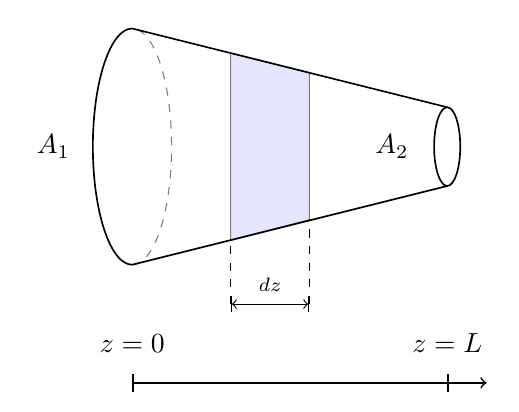
\begin{tikzpicture}
			\draw [fill=blue!20!white,opacity=0.5] (2.25,2.44) -- (2.25,0.57) -- (1.25,0.31) -- (1.25,2.69) -- cycle;%smmall triangle
			\draw[dashed,color=gray] (0,0) arc (-90:90:0.5 and 1.5);% right half of the left ellipse
			\draw[semithick] (0,0) -- (4,1);% bottom line
			\draw[semithick] (0,3) -- (4,2);% top line
			\draw[semithick] (0,0) arc (270:90:0.5 and 1.5);% left half of the left ellipse
			\draw[semithick] (4,1.5) ellipse (0.166 and 0.5);% right ellipse
			\draw (-1,1.5) node {$A_1$};
			\draw (3.3,1.5) node {$A_2$};
			\draw[|-,semithick] (0,-1.5) -- (4,-1.5);
			\draw[|->,semithick] (4,-1.5) -- (4.5,-1.5);
			\draw (0,-1) node {$z=0$};
			\draw (4,-1) node {$z=L$};
			\draw (1.75,-0.25) node{\scriptsize $ dz $}; %a number
			\draw[|<->|] (1.25,-0.5) -- (2.25,-0.5); %lenght indicator
			\draw[dashed] (1.25,-0.5) -- (1.25,0.3); %dashed line
			\draw[dashed] (2.25,-0.5) -- (2.25,0.58); %dashed line
		\end{tikzpicture}
		\caption{Control volume for deriving partial differential equation for unsteady, quasi-one-dimensional flow}
		\label{fig: control_volume}
	\end{figure}
	
	This control volume is a slice of an extractor, where the infinitesimal thickens of the slice is $dz$. On the left side of the control volume, consistent with the quasi-one-dimensional assumptions, the density, velocity, pressure and internal energy denoted by $\rho_f$, $V$, $P$, and $e$, respectively, are uniform over the are $A$. Similarly, on the right side of the control volume, the density, velocity, pressure, and internal energy $\rho_f+d\rho_f$, $V+dV$, $P+dP$, and $e+de$, respectively, are uniform over the area available for fluid phase $A_f+dA_f$. Applied to the control volume in Fig. \ref{fig: control_volume}, the volume integral in Eq. \ref{EQ: Continuity_integral_general} becomes, in the limit as $dz$ becomes very small,
	
	{\footnotesize
		\begin{equation}
			\cfrac{\partial}{\partial t} \iiint_{\mathcal{V}_f} \rho_f d\mathcal{V}_f = \cfrac{\partial}{\partial t}\left( \rho_f A_f dz \right)
			\label{EQ: Cont_Simpl_Vol}
		\end{equation}
	}

	where $A~dz$ is the volume of the control volume in the limit of $dz$ becoming vanishingly small. The surface integral in Eq. \ref{EQ: Continuity_integral_general} becomes
	
	{\footnotesize
		\begin{equation}
			\iint_S \rho_f \textbf{V} \cdot \textbf{dS} = -\rho_f V A_f + (\rho_f+d\rho_f)(V+dV)(A_f+dA_f)
		\end{equation}
	}

	where the minus sign on the leading term on the right-hand side is due to the vectors $\textbf{V}$ and $\textbf{dS}$ pointing in opposite directions over the left of the control volume, and hence the dot product is negative. Expending the triple product term 
	 
	{\footnotesize
		\begin{align}
			&\iint_S \rho_f \textbf{V} \cdot \textbf{dS} = -\rho_f V A_f + \rho_f V A_f + \rho_f V dA_f + \rho_f A_f dV \nonumber \\ 
			&+ \rho_f dV dA_f + V A_f d\rho_f + V d\rho_f dA + A_f d\rho_f dV + d\rho_f dV dA_f
			\label{EQ: Triple_Prod_Cont_Surf}
		\end{align}
	}
	
	In the limit as $dz$ becomes very small, the terms involving products of the differential in Eq. \ref{EQ: Triple_Prod_Cont_Surf}, sych as $\rho_f dV dA_f,~d\rho_f dV dA_f$, go to zero much faster than those terms involving only one differential. Hence, all terms involving products of differentials can be dropped, yielding in the limit as $dz$ becomes very small
	
	{\footnotesize
		\begin{equation}
			\iint_S \rho_f \textbf{V} \cdot \textbf{dS} = \rho_f V dA_f + \rho_f A_f dV + V A_f d\rho_f 
			\label{EQ: Cont_Simpl_Surf}
		\end{equation}
	}

	Substituting Eqs. \ref{EQ: Cont_Simpl_Vol} and \ref{EQ: Cont_Simpl_Surf} into \ref{EQ: Continuity_integral_general}, we have
	
	{\footnotesize
		\begin{equation}
			\cfrac{\partial \left( \rho_f A_f \right)}{\partial t} + \cfrac{\partial \left( \rho_f A_f V \right)}{\partial z} = 0
			\label{EQ: Conservative_continuity}
		\end{equation}
	}
	
	Above partial differential equation form of the continuity equation suitable for unsteady, quasi-one-dimensional flow. It ensures that mass is conserved for this mode of the flow. The $A_f(z)$ is an arbitrary function, which describe change of the cross-section of an extractor. The function $A_f(z)$ can be defined as $A_f(z) = \textbf{A} \varepsilon(z)$, where $\varepsilon$ is the bed porosity and $\textbf{A}$ is the cross-section of an empty extractor.
	
	{\footnotesize
		\begin{equation}
			\cfrac{\partial \left( \rho_f \textbf{A} \varepsilon (z) \right)}{\partial t} + \cfrac{\partial \left( \rho_f \textbf{A} \varepsilon (z) V \right)}{\partial z} = 0
		\end{equation}
	}
	The equation can be simplified by cancel out a constant $\textbf{A}$
	
	{\footnotesize
		\begin{equation}
			\cfrac{\partial \left( \rho_f \varepsilon (z) \right)}{\partial t} + \cfrac{\partial \left( \rho_f \varepsilon (z) V \right)}{\partial z} = 0
		\end{equation}
	}
	
	If so called superficial velocity is defined $u=\varepsilon V$, the mass continuity becomes
	
	{\footnotesize
		\begin{equation}
			\cfrac{\partial \left( \rho_f \varepsilon (z) \right)}{\partial t} + \cfrac{\partial \left( \rho_f u \right)}{\partial z} = 0
			\label{EQ: Mass_Continuity}
		\end{equation}
	}
	
	\hrule
	
	\subsubsection{Transport of a species}
	
	The transport of a chemical species, in this case a solute, can be described by analogous equation to the Eq. \ref{EQ: Continuity_integral_general} with additional terms on the right-hand side. The first term on the right-hand side describes that a substance goes from high density regions to low density regions and is based on the Fick's law ${\footnotesize\left( J_{diff} = D\cfrac{\partial C_f}{\partial z} \right)}$. The other term correspond for the mass transfer between solid and fluid phases, which is treated as a source term.
	
	{\footnotesize
		\begin{equation}
			\cfrac{\partial}{\partial t} \iiint_{\mathcal{V}_f} C_f d\mathcal{V}_f + \iint_S C_f \textbf{V} \cdot \textbf{dS} = \iint_S J_{diff} \cdot \textbf{n}~\textbf{dS} + \cfrac{\partial}{\partial t} \iiint_{\mathcal{V}_s} C_s d\mathcal{V}_s
			\label{EQ: Integral_Mass_Species_general}
		\end{equation}
	}
	
	Similarly to the continuity equation, in the limit as $dz$ becomes very small
	
	{\footnotesize
		\begin{align}
			\cfrac{\partial}{\partial t} \iiint_{\mathcal{V}_f} C_f d\mathcal{V}_f &= \cfrac{\partial}{\partial t}\left( C_f A_f dz \right) \\
			\cfrac{\partial}{\partial t} \iiint_{\mathcal{V}_s} C_s d\mathcal{V}_s &= \cfrac{\partial}{\partial t}\left( C_s A_s dz \right)
		\end{align}
	}

	The surface integrals in the limit of $dz$ becomes
	
	{\footnotesize
		\begin{equation}
			\iint_S C_f \textbf{V} \cdot \textbf{dS} = C_f V dA_f + C_f A_f dV + V A_f dC_f 
		\end{equation}
	}
	
	From the Divergence theorem in multi-variable calculus, we have
	
	{\footnotesize
		\begin{equation}
			\iint_S J_{diff} \cdot \textbf{n}~\textbf{dS} = \iiint_{\mathcal{V}_f} \nabla J_{diff} dV_f = \nabla \iiint_{\mathcal{V}_f} J_{diff} dV_f = \nabla \left( J_{diff} A_f dz \right)
		\end{equation}
	}
	
	By substituting the equations derived above into Eq. \ref{EQ: Integral_Mass_Species_general} we obtain
	
	{\footnotesize
		\begin{equation}
			\cfrac{\partial \left( C_f A_f \right)}{\partial t} + \cfrac{\partial \left( C_f A_f V \right)}{\partial x} = \cfrac{\partial \left( C_s A_s \right) }{\partial t} + \cfrac{\partial \left( J_{diff} A_f \right) }{\partial z}
		\end{equation}
	}

	By defining $A_f = A \cdot \varepsilon$, $A_s = A \cdot \left( 1-\varepsilon \right)$ and $u=V \cdot \varepsilon$, and assuming that $A$ is constant, the above equation becomes
	
	{\footnotesize
		\begin{equation}
			\cfrac{\partial \left( C_f \varepsilon \right)}{\partial t} + \cfrac{\partial \left( C_f u\right)}{\partial x} = \cfrac{\partial \left( C_s (1-\varepsilon) \right) }{\partial t} + \cfrac{\partial \left( J_{diff} \varepsilon \right) }{\partial z}
		\end{equation}
	}

	By expanding above equation, splitting variable and assuming that ${\footnotesize \cfrac{\partial \varepsilon}{\partial t}=0}$ we get
	
	{\footnotesize
		\begin{equation}
			\cfrac{\partial C_f}{\partial t} + \cfrac{u}{\varepsilon} \cfrac{\partial C_f}{\partial z} + \cfrac{C_f}{\varepsilon} \cfrac{\partial u}{\partial z} = \cfrac{1-\varepsilon}{\varepsilon} \cfrac{\partial C_s}{\partial t} + \cfrac{D}{\varepsilon} \cfrac{\partial C_f}{\partial z} \cfrac{\partial \varepsilon}{\partial z} + \cfrac{\partial}{\partial z} \left( D \cfrac{\partial C_f}{\partial z} \right)
		\end{equation}
	}
	
	The equation can be further simplified if $\cfrac{\partial u}{\partial z} = \cfrac{\partial \varepsilon}{\partial z} = D = 0$, which corresponds to the assumptions of constant velocity along the bed( which might be a case of isothermal and low-mach number flow), constant porosity( which comes from the assumption of constant area for both solid and fluid phase) and no radial diffusion.
	
	{\footnotesize
		\begin{equation}
			\cfrac{\partial C_f}{\partial t} + \cfrac{u}{\varepsilon} \cfrac{\partial C_f}{\partial z}  = \cfrac{1-\varepsilon}{\varepsilon} \cfrac{\partial C_s}{\partial t} 
			\label{EQ: Simplified_Species_Conservation}
		\end{equation}
	}

	The Eq. \ref{EQ: Simplified_Species_Conservation} is equivalent to the equation presented by \citet{Reverchon1996}.
	
	\hrule
	
	\subsubsection{Momentum conservation}
	
	Similarly to the mass conservation, the momentum conservation is derived for inviscid fluid with no body forces
	
	{\footnotesize
		\begin{equation}
			\cfrac{\partial}{\partial t} \iiint_{\mathcal{V}_f} \left( \rho_f V_z \right) d\mathcal{V}_f + \iint_S \left( \rho_f V_z \textbf{V} \right) \textbf{dS} = \iint_S \left( P dS \right)_z
			\label{EQ: Momentum_Integral_Form}
		\end{equation}
	}
	where $V_z$ is the $z$ component of the velocity.

	We the momentum conservation to the shaded control volume in Fig. \ref{fig: control_volume}, the integrals on the left side are evaluated in the same manner as discussed above in the regard to the continuity equation. That is,
	
	{\footnotesize
		\begin{equation}
			\cfrac{\partial}{\partial t} \iiint_{\mathcal{V}_f} \left( \rho_f V_z \right) d \mathcal{V}_f = \cfrac{\partial}{\partial t} \left( \rho_f V A_f dz \right)
			\label{EQ: Force_Continuity_Monenmtum}
		\end{equation}equation
	}
	
	and 
	
	{\footnotesize
		\begin{equation}
			\iint_S \left( \rho_f V_z \textbf{V} \right) dS = -\rho_f V^2 + \left( \rho_f + d \rho_f \right) \left( V+dV \right)^2 \left( A+dA \right)
		\end{equation}
	}
	
	\begin{figure}[h]
		\centering
		\includegraphics[width=\columnwidth]{Forces.pdf}
		\caption{The forces in the $z$ direction acting on the control volume}
		\label{fig: Forces_Momentum_Control_Volume}
	\end{figure}
	
	The evaluation of the pressure force term on the right side of Eq. \ref{EQ: Momentum_Integral_Form} can be understood based on the Fig. \ref{fig: Forces_Momentum_Control_Volume}. Here, the $z$ components of the vector $PdS$ are shown on all four side of the control volume. Remember that $\textbf{dS}$ is assumed to points away from the control volume; hence  any $z$ component $\left( PdS \right)_z$ that acts toward the left (in the negative $z$ direction) is a negative quantity, and any $z$ component that acts toward the right (in the positive $z$ direction) is a positive quantity. Also note that the $z$ component of $P\textbf{dS}$ acting on the top and the bottom inclined faces of the control volume in Fig. \ref{fig: Forces_Momentum_Control_Volume} can be expressed as the pressure $P$ acting on the component of the inclined are projected perpendicular to the $z$ direction, $dA_f/2$; hence, the contribution of each inclined face (top or bottom) to the pressure integral in Eq. \ref{EQ: Momentum_Integral_Form} is $-P(dA_f/2)$. All together, the right-hand side of Eq. \ref{EQ: Momentum_Integral_Form} is expressed as follows:
	
	{\footnotesize
		\begin{equation}
			\iint \left( PdS \right)_z = -PA_f + (P+dP)(A+dA_f)-2P\cfrac{dA_f}{2}
			\label{EQ: Force_Integral_Varying_Cross_Section}
		\end{equation}
	}
	
	Substituting Eqs. \ref{EQ: Force_Continuity_Monenmtum} to \ref{EQ: Force_Integral_Varying_Cross_Section} into Eq. \ref{EQ: Momentum_Integral_Form}, we have
	
	{\footnotesize
		\begin{align}
			& \cfrac{\partial}{\partial t} \left( \rho_f V A_f dz \right) - \rho_f V^2 A_f + (\rho_f + d\rho_f)(V+dV)^2(A_f+dA_f)  \nonumber \\
			&= PA_f - (P+dP)(A+dA_f)+PdA_f
		\end{align}
	}
	
	Cancelling like terms and ignoring products of differentials, equation above becomes in the limit $dz$ becoming  very small
	
	{\footnotesize
		\begin{equation}
			\cfrac{\partial}{\partial t} \left( \rho_f V A_f dz \right) + d\left( \rho_f V^2 A_f \right) = -A dP
		\end{equation}
	}

	Dividing above equation by $dz$ and taking the limit as $dz$ goes to zero, we obtain
	
	{\footnotesize
		\begin{equation}
			\cfrac{\partial \left( \rho_f V A_f \right)}{\partial t} + \cfrac{\partial \left( \rho_f V^2 A_f \right)}{\partial z} = -A_f \cfrac{\partial P}{\partial z}
			\label{EQ: Conservative_Momentum}
		\end{equation}
	}

	The Eq. \ref{EQ: Conservative_Momentum} can be expanded further by assuming that $A_f = \textbf{A}\varepsilon$ 
	
	{\footnotesize
		\begin{equation}
			\cfrac{\partial \left( \rho_f V \textbf{A} \varepsilon \right) }{\partial t} + \cfrac{\partial \left( \rho_f V^2 \textbf{A} \varepsilon \right) }{\partial z} = - 	\textbf{A} \varepsilon \cfrac{\partial P}{\partial t}
		\end{equation}
	}

	The equation can be further simplified by assuming that the cross-section of an extractor $\textbf{A}$ is constant and cancel out
	
	{\footnotesize
		\begin{equation}
			\cfrac{\partial \left( \rho_f V \varepsilon \right) }{\partial t} + \cfrac{\partial \left( \rho_f V^2 \varepsilon \right) }{\partial z} = - \varepsilon 	\cfrac{\partial P}{\partial t}
		\end{equation}
	}

	If the superficial velocity $u=\varepsilon V$ is introduced, then the momentum conservation becomes
	
	{\footnotesize
		\begin{equation}
			\cfrac{\partial \left( \rho_f u \right)}{\partial z} + \cfrac{\partial \left( \rho_f u^2/\varepsilon \right) }{\partial z} = -\varepsilon \cfrac{\partial 	P}{\partial z}
		\end{equation}
	}

	Eq. \ref{EQ: Conservative_Momentum} represents the conservative form of the momentum equation for the quasi-one-dimensional flow. The equivalent non-conservative form can be obtained by multiplying the continuity equation by $V$ and subtracting it from Eq. \ref{EQ: Conservative_Momentum}
	
	{\footnotesize
		\begin{equation}
			\cfrac{\partial \left( \rho_f V A_f \right)}{\partial t} - V\cfrac{ \partial \left( \rho_f A_f \right) }{\partial t} + \cfrac{\left( \rho_f V^2 A_f 	\right)}{\partial z} - V \cfrac{\left( \rho_f V A_f \right)}{\partial z} = -A_f \cfrac{\partial P}{\partial z}
		\end{equation}
	}
	
	Expanding the derivatives on the left-hand size of above equation and cancelling like terms, gives

	{\footnotesize
		\begin{equation}
			\rho_f A_f \cfrac{\partial V}{\partial t} + \rho_f A_f V \cfrac{\partial V}{\partial z} = -A_f \cfrac{\partial P}{\partial z}
		\end{equation}
	}

	Dividing above equation by $A_f$ the non-conservative form of the momentum can be obtained
	
	{\footnotesize
		\begin{equation}
			\rho_f \cfrac{\partial V}{\partial t} + \rho_f V \cfrac{\partial V}{\partial z} = -\cfrac{\partial P}{\partial z}
			\label{EQ: Non-conservative_Momentum}
		\end{equation}
	}

	The Eq. \ref{EQ: Non-conservative_Momentum} is stylistically the same as the general momentum conservation for one-dimensional flow with no-body forces. The momentum equation can be expressed in terms of superficial velocity $u=V\varepsilon$. 
	
	{\footnotesize
		\begin{equation}
			\rho_f \cfrac{\partial \left(u / \varepsilon \right)}{\partial t} + \rho_f \cfrac{u}{\varepsilon} \cfrac{\partial \left( u / \varepsilon \right)}{\partial z} = - \cfrac{\partial P}{\partial z}
		\end{equation}
	}

	By expanding all the terms of equation above, we get
	
	{\footnotesize
		\begin{equation}
			\cfrac{\rho_f}{\varepsilon} \cfrac{\partial u}{\partial t} + \rho_f u \cfrac{\partial \varepsilon^{-1}}{\partial t} + \rho_f \cfrac{u}{\varepsilon} \cfrac{1}{\varepsilon} \cfrac{\partial u}{\partial z} + \rho_f \cfrac{u}{\varepsilon} u \cfrac{\partial \varepsilon^{-1} }{\partial z} = - \cfrac{\partial P}{\partial z}
		\end{equation}
	}
	
	If the bed is not compressible and doesn't change its properties during the batch, then ${\footnotesize\cfrac{\partial \varepsilon}{\partial t}=0}$
	
	{\footnotesize
		\begin{equation}
			\cfrac{\rho_f}{\varepsilon} \left( \cfrac{\partial u}{\partial t} + \cfrac{u}{\varepsilon} \cfrac{\partial u}{\partial z} + u^2 \cfrac{\partial \varepsilon^{-1}}{\partial z} \right) = -\cfrac{\partial P}{\partial z}
		\end{equation}
	}

	If the porosity is constant along an extractor, then the momentum conservation equation becomes
	
	{\footnotesize
		\begin{equation}
			\cfrac{\rho_f}{\varepsilon} \left( \cfrac{\partial u}{\partial t} + \cfrac{u}{\varepsilon} \cfrac{\partial u}{\partial z} \right) = -\cfrac{\partial P}{\partial z}
			\label{EQ: Non-conservative_Momentum_Const_Porosity}
		\end{equation}
	}

	The Eq. \ref{EQ: Non-conservative_Momentum_Const_Porosity} represents non-conservative form of the momentum equation for quasi-one-dimensional flow with no body forces and constant porosity.
	
	\hrule
	
	\subsubsection{Energy conservation}
	
	Let's consider the integral form of the energy equation for adiabatic flow with no body forces and no viscous effects
	
	{\footnotesize
		\begin{equation}
			\cfrac{\partial}{\partial} \iiint_{\mathcal{V}_f} \rho_f \left( e_f + \cfrac{V^2}{2} \right) d\mathcal{V}_f + \iint_S \rho_f \left( e_f + \cfrac{V^2}{2} \right) \textbf{V} \cdot \textbf{dS} = - \iint_S \left( P\textbf{V} \right) \cdot \textbf{dS}
			\label{EQ: Energy_equation_integral}
		\end{equation}
	}

	Applied to the shaded control volume in Fig. \ref{fig: control_volume}, and keeping in mind the pressure forces shown in Fig. \ref{fig: Forces_Momentum_Control_Volume}, Eq. \ref{EQ: Energy_equation_integral} becomes
	
	{\footnotesize
		\begin{align}
			&\cfrac{\partial}{\partial t} \left[ \rho_f \left( e_f + \cfrac{V^2}{2} \right) A_f dz \right] - \rho_f \left( e_f + \cfrac{V^2}{2} \right) V A_f \nonumber \\
			&+ \left( \rho_f + d\rho_f \right) \left[ e_f + de_f + \cfrac{\left( V + dV \right)^2}{2} \right] \left( V+fV \right) \left( A_f+dA_f \right) \nonumber \\
			&= - \left[ -PVA_f + \left(P+dP\right) \left(V+dV\right) \left(A_f+dA_f\right) - 2\left( PV\cfrac{dA_f}{2} \right) \right]
		\end{align}
	}
	
	Neglecting products of differential and cancelling like terms, the above equation becomes
	
	{\footnotesize
		\begin{equation}
			\cfrac{\partial}{\partial t} \left[ \rho_f \left( e_f + \cfrac{V^2}{2} \right) A_f dz \right] + d\left( \rho_f r_f A_f \right) + \cfrac{ \left( \rho_f V^3 A_f \right) }{2} = -d \left( P A_f V \right)
		\end{equation}
	}

	or
	
	{\footnotesize
		\begin{equation}
			\cfrac{\partial}{\partial t} \left[ \rho_f \left( e_f + \cfrac{V^2}{2} \right) A_f dz \right] + d \left[ \rho_f \left( e_f \cfrac{V^2}{2} \right) VA_f \right] = - d\left( P A_f V \right)
		\end{equation}
	}

	Taking the limit as $dz$ approaches zero, the equation above becomes the following partial differential equation
	
	{\footnotesize
		\begin{equation}
			\cfrac{\partial \left[ \rho_f \left( e_f + V^2 / 2 \right) A \right]}{\partial t} + \cfrac{\partial \rho_f \left( e_f + V^2 / 2 \right)VA_f}{\partial z} = -\cfrac{\partial \left( P A_f V \right)}{\partial z}
			\label{EQ: Energy_equation_conservative_total}
		\end{equation}
	}
	
	Equation \ref{EQ: Energy_equation_conservative_total} is the conservation form of the energy expressed in terms of the total energy $e~+~V^2/2$, appropriate for unsteady, quasi-one-dimensional flow. The energy equation can be expressed in terms of internal energy if Eq. \ref{EQ: Conservative_Momentum} is multiplicated by $V$ and then subtracted from Eq. \ref{EQ: Energy_equation_conservative_total}
	
	{\footnotesize
		\begin{equation}
			\cfrac{\partial \left( \rho_f e_f A_f \right) }{\partial t} + \cfrac{\partial \left( \rho_f  e_f V A_f \right)}{\partial z} = -P \cfrac{\partial A_f V}{\partial z}
			\label{EQ: Energy_conservative_internal}
		\end{equation}
	}
	
	The equation above is the conservation form of the energy equation expressed in terms of internal energy $e_f$ suitable for quasi-one-dimensional flow. The non-conservative for is then obtained by multiplying the continuity equation \ref{EQ: Conservative_continuity}, by $e_f$ and substructing it from \ref{EQ: Energy_conservative_internal}, yielding 
	
	{\footnotesize
		\begin{equation}
			\rho_f A_f \cfrac{\partial e_f}{\partial t} + \rho_f A_f V \cfrac{\partial e_f}{\partial z} = - P \cfrac{\partial (A_f V) }{\partial z}
		\end{equation}
	}
	
	Expanding right-hand side and dividing by $A_f$, the above equation becomes 
	
	{\footnotesize
		\begin{equation}
			\rho_f \cfrac{\partial e_f}{\partial t} + \rho_f V \cfrac{\partial e_f}{\partial z} = -P \cfrac{V}{A_f} \cfrac{\partial A_f}{\partial z}
		\end{equation}
	}

	or
	
	{\footnotesize
		\begin{equation}
			\rho_f \cfrac{\partial e_f}{\partial t} + \rho_f V \cfrac{\partial e_f}{\partial z} = -P \cfrac{\partial V}{\partial z} - P V \cfrac{\partial (ln~A_f)}{\partial z}
			\label{EQ: Energy_equation_nonconservative}
		\end{equation}
	}
	
	Equation \ref{EQ: Energy_equation_nonconservative} is the non-conservative for of the energy equation expressed in therms of internal energy, appropriate to unsteady quasi-one-dimensional flow. The reason for obtaining the energy equation in the form of Eq. \ref{EQ: Energy_equation_nonconservative} is that, for a calorically perfect gas, it leads directly to a form of the energy equation in therms of temperature $T$. For calorically perfect gas ${\footnotesize e_f=C_vT}$
	
	\hrule
	
	{\footnotesize
		\begin{equation}
			\cfrac{\partial \left( \rho_f e_f A_f \right) }{\partial t} + \cfrac{\partial \left( \rho_f  e_f V A_f \right)}{\partial z} = -P \cfrac{\partial A_f V}{\partial z} + \cfrac{\partial}{\partial z} \left( k \cfrac{\partial T}{\partial z} \right)
		\end{equation}
	}
	
	{TODO: \color{red}finish derivation of energy equation for real gas and introduce homogenous version of the energy equation}
	
	
	
	
	
	
	
	
	
	
	
	
	
	
\end{document}